\documentclass[12pt,letterpaper,twocolumn,openany,nodeprecatedcode,bg=none]{dndbook}
\usepackage[english]{babel}
\usepackage[utf8]{inputenc}
\usepackage{longtable,booktabs,array}
\usepackage{calc}
\usepackage{etoolbox}
\usepackage{caption}
\AtBeginEnvironment{longtable}{\small}

% Fix for Pandoc 3.1.7+ image handling
\providecommand{\pandocbounded}[1]{#1}

% Pandoc's compact list helper
\providecommand{\tightlist}{%
  \setlength{\itemsep}{0pt}\setlength{\parskip}{0pt}}

% Remove "Figure N:" prefix from captions
\captionsetup{labelformat=empty}

% Remove section numbering
\setcounter{secnumdepth}{0}

\begin{document}

\title{Wizard}
\author{Class Handbook}
\date{}
\maketitle

\onecolumn

\emph{Your trusty class handbook for the Old Scrolls roleplaying game.}

\clearpage

\begin{figure}
\centering
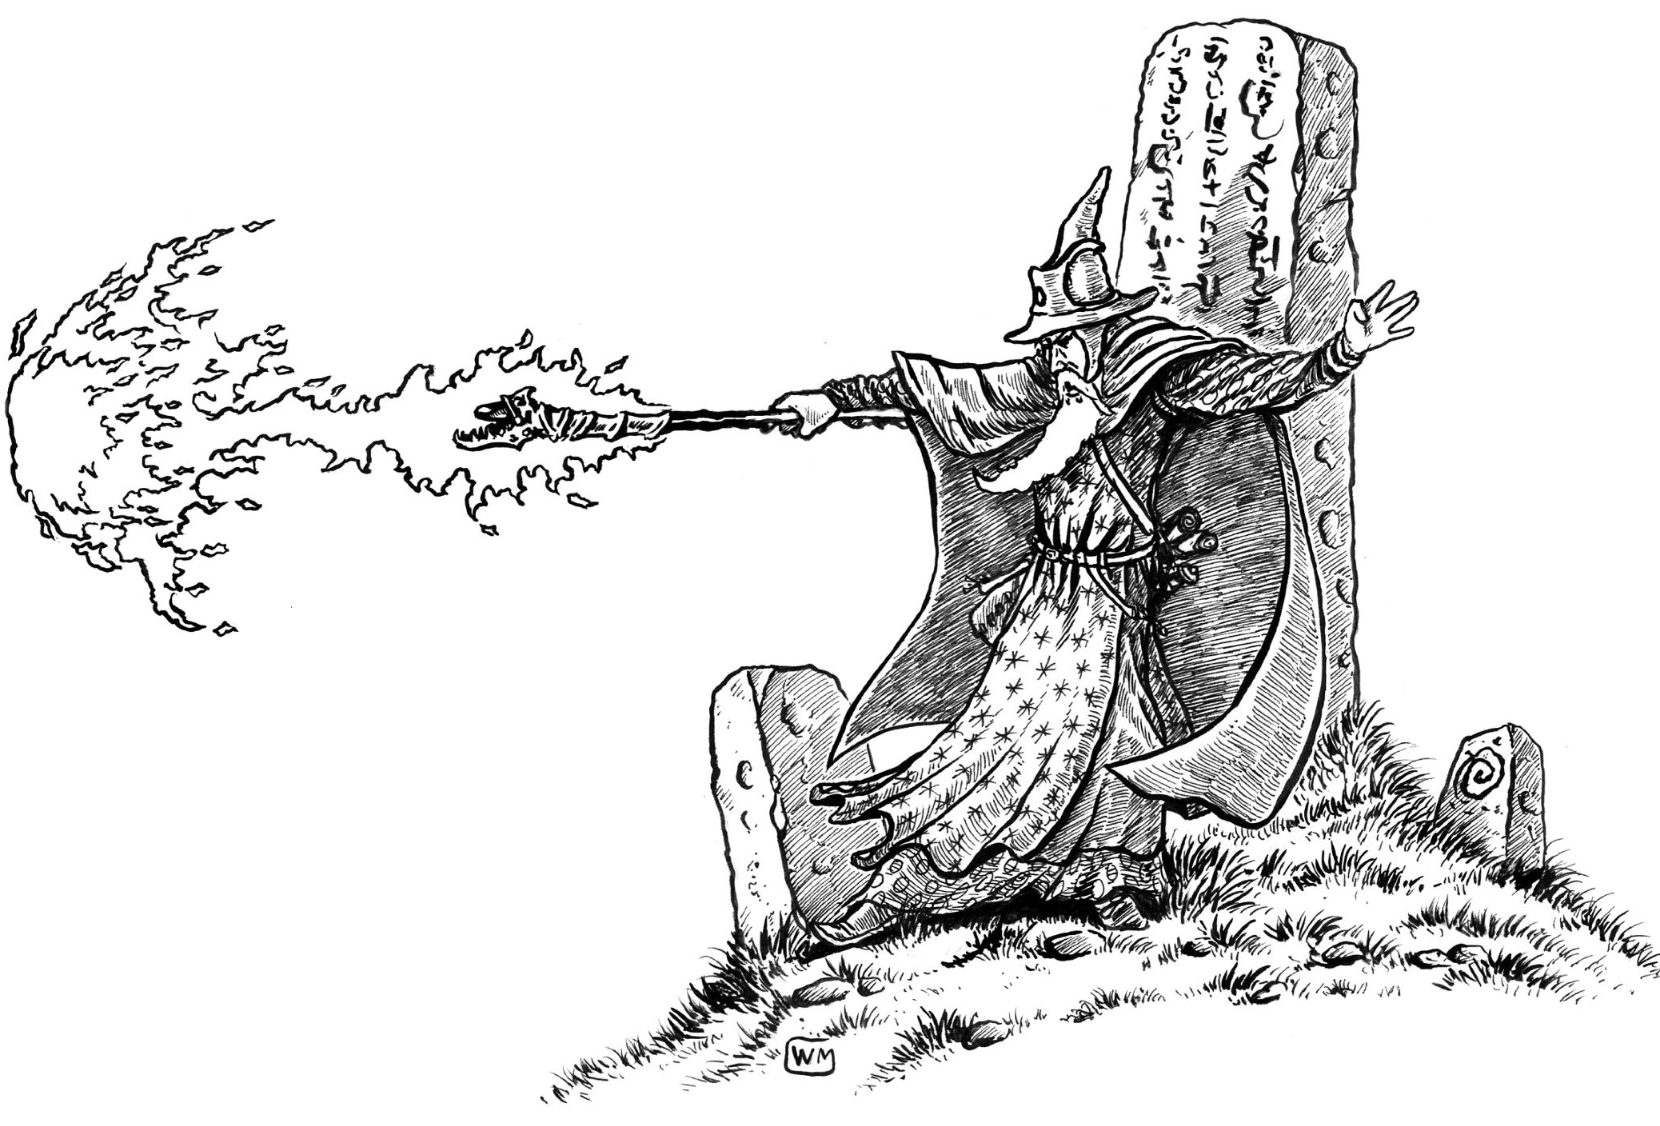
\includegraphics[width=0.7\linewidth,height=\textheight,keepaspectratio]{classicWizard.png}
\caption{\emph{A wizard casts fireball.}}
\end{figure}

\begin{figure}
\centering
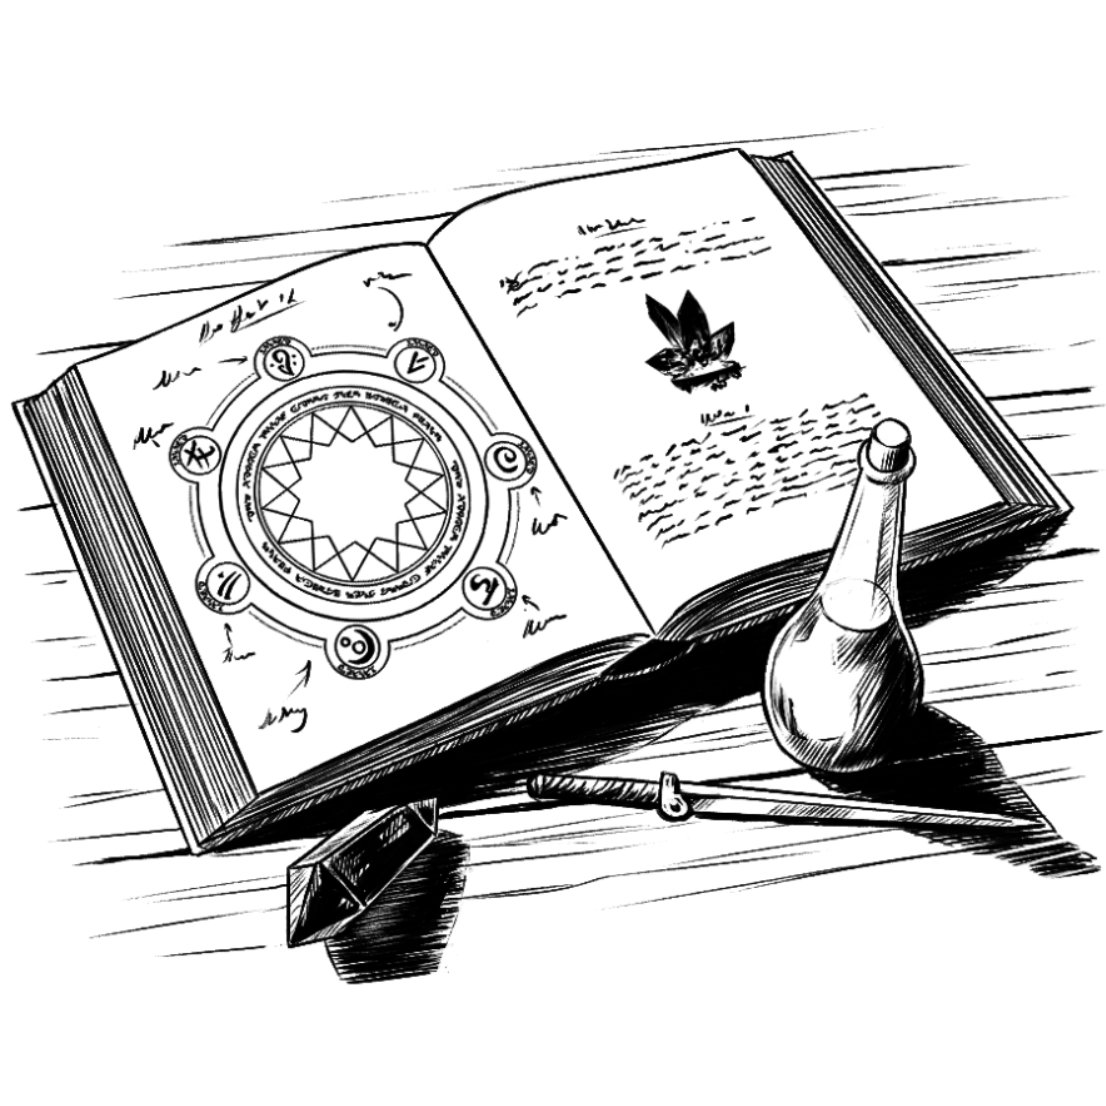
\includegraphics[width=0.7\linewidth,height=\textheight,keepaspectratio]{spellbook.png}
\caption{\emph{Every wizard needs a spellbook.}}
\end{figure}

\clearpage

\section{Wizard}\label{wizard}

As a wizard, you take a generalist approach to magic. Rather than
focusing on one specific niche of magic, you dabble in harnessing
various effects, learning spells as they suit your needs.

\subsection{Core Wizard Traits}\label{core-wizard-traits}

\begin{longtable}[]{@{}
  >{\raggedright\arraybackslash}p{(\linewidth - 2\tabcolsep) * \real{0.2542}}
  >{\raggedright\arraybackslash}p{(\linewidth - 2\tabcolsep) * \real{0.7458}}@{}}
\toprule\noalign{}
\begin{minipage}[b]{\linewidth}\raggedright
\textbf{Primary Ability}
\end{minipage} & \begin{minipage}[b]{\linewidth}\raggedright
Intelligence
\end{minipage} \\
\midrule\noalign{}
\endhead
\bottomrule\noalign{}
\endlastfoot
\textbf{Hit Points} & 8 at 1st level, 6 per level gained after 1st \\
\textbf{Saving Throw Proficiencies} & Intelligence, Wisdom \\
\textbf{Skill Proficiencies} & Choose any 2 skills. If you choose a
skill you already have, you gain expertise with it. \\
\textbf{Weapon Proficiencies} & Choose 1: Blade, Blunt, Bow, Mechanical,
Polearm, and Shield \\
\textbf{Starting Equipment} & Padded Jacket, Staff, Spellbook, Robe \\
\end{longtable}

\subsection{Wizard Features}\label{wizard-features}

\begin{longtable}[]{@{}
  >{\raggedright\arraybackslash}p{(\linewidth - 8\tabcolsep) * \real{0.0575}}
  >{\raggedright\arraybackslash}p{(\linewidth - 8\tabcolsep) * \real{0.1264}}
  >{\raggedright\arraybackslash}p{(\linewidth - 8\tabcolsep) * \real{0.1724}}
  >{\raggedright\arraybackslash}p{(\linewidth - 8\tabcolsep) * \real{0.0920}}
  >{\raggedright\arraybackslash}p{(\linewidth - 8\tabcolsep) * \real{0.5517}}@{}}
\toprule\noalign{}
\begin{minipage}[b]{\linewidth}\raggedright
Level
\end{minipage} & \begin{minipage}[b]{\linewidth}\raggedright
Proficiency
\end{minipage} & \begin{minipage}[b]{\linewidth}\raggedright
Spells Prepared
\end{minipage} & \begin{minipage}[b]{\linewidth}\raggedright
Cantrips
\end{minipage} & \begin{minipage}[b]{\linewidth}\raggedright
Class Features
\end{minipage} \\
\midrule\noalign{}
\endhead
\bottomrule\noalign{}
\endlastfoot
1 & +2 & 2 & 2 & Spellcasting \\
2 & +2 & 3 & 2 & School Specialization \\
3 & +2 & 3 & 2 & Sculpt Spells \\
4 & +2 & 3 & 2 & Ability Score Improvement, School Specialization \\
5 & +3 & 4 & 3 & School Mastery \\
6 & +3 & 4 & 3 & School Specialization \\
7 & +3 & 4 & 3 & Spell Research \\
8 & +3 & 5 & 3 & Ability Score Improvement \\
9 & +4 & 5 & 3 & Spell Research \\
10 & +4 & 5 & 3 & Spell Mastery \\
\end{longtable}

\clearpage

\twocolumn

\subsection{Wizard Features}\label{wizard-features-1}

As a wizard, you gain the following class features when you reach the
specified levels. These features are listed on the Wizard Features
table.

\subsubsection{Level 1: Spellcasting}\label{level-1-spellcasting}

As a student of arcane magic, you have learned to cast spells.

\textbf{Spellcasting Ability.} Intelligence is the spellcasting ability
for wizard spells. If you make an attack roll with a spell, your bonus
is your Intelligence modifier plus your proficiency bonus. The saving
throw DC of your spells is 8 + your Intelligence modifier + your
proficiency bonus.

\textbf{Caster Level.} When you cast a spell, its effects might be
determined by your level. A spell's level must be less than or equal to
your level. Many spells have effects that scale, such as damage, based
on your level.

\textbf{Spells Known.} You start with three spells known. Pick or
randomly select three spells other than cantrips. When you gain a level,
you learn an additional spell from the wizard spell list. Some class
features grant you additional spells known.

\textbf{Spells Prepared.} You start with two spells prepared. You
prepare spells from among your spells known. You gain additional
prepared spells at levels 2, 5, and 8.

\textbf{Casting Spells.} When you cast a spell you have prepared, you
can't cast it again until you recharge that spell. You can recharge one
spell when you finish a short rest. You recharge all your spells when
you finish a long rest.

\textbf{Swapping Prepared Spells.} When you recharge a spell, you can
instead choose to prepare a different spell in its place from among
those you gained from this class or from wizard spells in spellbooks or
scrolls in your possession.

\textbf{Cantrips.} You know two wizard cantrips of your choice. Pick two
from the table given later in this section or roll to pick at random,
rerolling any duplicates. Unlike other spells, you retain the use of a
cantrip after you cast it. You do not have to recharge it. Each time you
gain a level, you can swap one or more of your cantrips for different
ones. You gain a third cantrip at level 5.

\subsubsection{Level 2: School
Specialization}\label{level-2-school-specialization}

As a wizard, you study and master the theories and mathematics behind
the forces used to create spell effects. As part of your studies, you
unlock deeper secrets. Choose a school specialization. You gain its
level 2 benefit.

At levels 4 and 6 you gain additional benefits from your chosen
specialization.

\subsubsection{Level 3: Sculpt Spells}\label{level-3-sculpt-spells}

When you cast a spell, you can choose to reduce the damage it does to
creatures of your choice to 0.

\subsubsection{Level 4: Ability Score
Improvement}\label{level-4-ability-score-improvement}

You gain a +1 bonus to two abilities of your choice.

\subsubsection{Level 4: School
Specialization}\label{level-4-school-specialization}

You gain your school specialization's level 4 benefit.

\subsubsection{Level 5: School Mastery}\label{level-5-school-mastery}

Choose a school of magic. You gain a +1 bonus to your attacks with
spells from that school and your save DC for those spells gains a +1
bonus.

\subsubsection{Level 6: School
Specialization}\label{level-6-school-specialization}

You gain your school specialization's level 6 benefit.

\subsubsection{Level 7: Spell Research}\label{level-7-spell-research}

Choose one of your spells that is not a cantrip, subject to restrictions
noted below. Your research allows you to customize the spell, making it
truly your own. Pick one of the following benefits. You can choose to
apply it to that spell when you cast it.

\begin{itemize}
\tightlist
\item
  \textbf{Echo Spell.} You may choose a spell with a level less than or
  equal to half your level. When you cast this spell, you may cast the
  spell twice, but a creature cannot be targeted by the spell more than
  once. If a creature would suffer the spell's effects more than once,
  the effects of only one casting apply to it. You treat your caster
  level as half your level when casting the spell.
\item
  \textbf{Elemental Infusion.} If the spell deals damage, you may change
  that damage's type to one of the following options: acid, cold, fire,
  lightning, or thunder. When you do so, you gain a bonus to damage
  rolls with that spell equal to your power during the turn on which you
  cast it.
\item
  \textbf{Temporal Weave.} You may cast the spell without using your
  action. Your caster level is reduced to 1 when casting the spell in
  this way. You may apply this benefit only to 1st level spells. You
  cannot use this feature while you are prevented from using magic
  actions.
\end{itemize}

You choose a second spell to gain this benefit at level 9.

\subsubsection{Level 8: Ability Score
Improvement}\label{level-8-ability-score-improvement}

You gain a +1 bonus to two abilities of your choice.

\subsubsection{Level 10: Spell Mastery}\label{level-10-spell-mastery}

When you cast a 1st-level spell, you can choose to cast it as if your
level was 1. If you do so, you can cast the spell again without needing
to recharge it.

\onecolumn

\subsection{Wizard Spell List}\label{wizard-spell-list}

The spell list for wizards is organized by level below. The tables are
numbered so that you can easily generate random spells of a given level
if you so desire.

\subsubsection{Cantrips}\label{cantrips}

\begin{longtable}[]{@{}ll@{}}
\toprule\noalign{}
d10 & Spell \\
\midrule\noalign{}
\endhead
\bottomrule\noalign{}
\endlastfoot
1 & Acid Bubble \\
2 & Death Echo \\
3 & Force Sphere \\
4 & Icy Grasp \\
5 & Hold Portal \\
6 & Light \\
7 & Minor Illusion \\
8 & Minor Telekinesis \\
9 & Siren's Call \\
10 & Vexing Swarm \\
\end{longtable}

\subsubsection{Level 1 (Tier 1)}\label{level-1-tier-1}

\begin{longtable}[]{@{}ll@{}}
\toprule\noalign{}
d8 & Spell \\
\midrule\noalign{}
\endhead
\bottomrule\noalign{}
\endlastfoot
1 & Arcane Slumber \\
2 & Flame Cage \\
3 & Flame Wave \\
4 & Fog Bank \\
5 & Illusory Image \\
6 & Mystic Eye \\
7 & Rolling Thunder \\
8 & Zephyr Steps \\
\end{longtable}

\subsubsection{Level 3 (Tier 2)}\label{level-3-tier-2}

\begin{longtable}[]{@{}ll@{}}
\toprule\noalign{}
d8 & Spell \\
\midrule\noalign{}
\endhead
\bottomrule\noalign{}
\endlastfoot
1 & Acid Rain \\
3 & Animate Armor \\
2 & Dragon Spirit \\
4 & Ethereal Cloak \\
5 & Necrotic Mote \\
6 & Spider Form \\
7 & Void of the Forsaken \\
8 & Wind Disk \\
\end{longtable}

\clearpage

\subsubsection{Level 5 (Tier 3)}\label{level-5-tier-3}

\begin{longtable}[]{@{}ll@{}}
\toprule\noalign{}
d9 & Spell \\
\midrule\noalign{}
\endhead
\bottomrule\noalign{}
\endlastfoot
1 & Arcane Aegis \\
2 & Fire Blast \\
3 & Flight \\
4 & Glyph of Warding \\
5 & Lightning Bolts \\
6 & Temporal Bubble \\
7 & Vapors of the Rotting Mire \\
8 & Water Breathing \\
\end{longtable}

\subsubsection{Level 7 (Tier 4)}\label{level-7-tier-4}

\begin{longtable}[]{@{}ll@{}}
\toprule\noalign{}
d4 & Spell \\
\midrule\noalign{}
\endhead
\bottomrule\noalign{}
\endlastfoot
1 & Arcane Eye \\
2 & Worm Hole \\
3 & Fiery Redoubt \\
4 & Ice Storm \\
\end{longtable}

\subsubsection{Level 9 (Tier 5)}\label{level-9-tier-5}

\begin{longtable}[]{@{}ll@{}}
\toprule\noalign{}
d2 & Spell \\
\midrule\noalign{}
\endhead
\bottomrule\noalign{}
\endlastfoot
1 & Conjured Blizzard \\
2 & Crimson Chains \\
\end{longtable}

\twocolumn

\subsection{School Specialization}\label{school-specialization}

You choose a technique of magic that reflects your focused area of
study.

\subsubsection{Abjurer}\label{abjurer}

You study magic that protects you and wards away threats.

\textbf{Level 1.} You gain the arcane shield cantrip. You gain it in
addition to the cantrips you normally gain from the wizard class and
always have it prepared.

\textbf{Level 4.} You gain arcane shield's level 4 benefit.

\textbf{Level 6.} You gain arcane shield's level 6 benefit.

\subsubsection{Arcane Archer}\label{arcane-archer}

You study how to suffuse arrows with powerful magic.

\textbf{Level 1.} You gain proficiency with bows. As an attack action,
you can make an attack with a bow that gains a bonus to its damage roll
equal to your spellcasting modifier.

\textbf{Level 4.} When you attack with a bow, you can change its damage
type to your choice of acid, cold, fire, lightning, or thunder.

\textbf{Level 6.} As a magic attack action, you can make a bow attack
and cast a wizard cantrip, or you can make two bow attacks.

\subsubsection{Conjurer}\label{conjurer}

You study magic that creates objects and summons creatures from the
planes.

\textbf{Level 1.} You gain the conjure atronach cantrip. You gain it in
addition to the cantrips you normally gain from the wizard class and
always have it prepared.

\textbf{Level 4.} You gain conjure elemental's level 4 benefit.

\textbf{Level 6.} You gain conjure elemental's level 6 benefit.

\subsubsection{Evoker}\label{evoker}

You study magic that unleashes powerful, destructive forces.

\textbf{Level 1.} You gain the spell storm cantrip. You gain it in
addition to the cantrips you normally gain from the wizard class and
always have it prepared.

\textbf{Level 4.} You gain spell storm's level 4 benefit.

\textbf{Level 6.} You gain spell storm's level 6 benefit.

\subsubsection{Restorer}\label{restorer}

You study restoration magic, the powers that sustains and fortifies
others.

\textbf{Level 1.} As a magic action, you can exhaust a prepared spell
and cause a creature within 60 feet to regain 1d8 hit points per level +
your spellcasting modifier.

\textbf{Level 4.} When you cast a wizard spell that is not a cantrip, a
creature of your choice within melee range regains hit points equal to
your level + your spellcasting modifier.

\textbf{Level 6.} Your level 4 benefit can now apply to up to three
creatures within melee range.

\subsubsection{Transmuter}\label{transmuter}

You study magic that allows you to alter living things and inert
objects.

\textbf{Level 1.} You gain the modify self cantrip. You gain it in
addition to the cantrips you normally gain from the wizard class and
always have it prepared.

\textbf{Level 4.} You gain modify self's level 4 benefit.

\textbf{Level 6.} You gain modify self's level 6 benefit.

\clearpage

\section{Wizard Spells}\label{wizard-spells}

\subsection{Acid Bubble}\label{acid-bubble}

\textbf{Level:} Cantrip

\textbf{Casting Time:} Magic Attack Action

\textbf{Duration:} Instantaneous

You create an acidic bubble within range that pops and splashes acid
over a 5-foot-radius sphere centered on a point you choose. Pick a
number of creatures in that area up to half your level. Each chosen
creature takes acid damage equal to your level + your spellcasting
modifier.

\subsection{Animate Armor}\label{animate-armor}

\textbf{Level:} 3

\textbf{Casting Time:} Magic Action

\textbf{Range:} Self

\textbf{Duration:} Concentration

You touch a suit of armor and empower it with arcane force, allowing it
to move on its own. It is a size Medium construct. It has AC 18 and hit
points equal to your level times 4. If it needs to make a saving throw
or check, it uses the bonus you would use for that test.

Friendly creatures within melee range of the guardian can use the higher
of AC 20 or their AC against ranged attacks. Once during your turn, you
can move the guardian up to 30 feet. At the end of each of your turns,
up to one creature in melee range of the guardian takes 1d6 + your
spellcasting modifier + half your level force damage.

\subsection{Arcane Aegis}\label{arcane-aegis}

\textbf{Level:} 5

\textbf{Casting Time:} Magic Action

\textbf{Range:} 5 feet

\textbf{Duration:} Concentration

For the duration, friendly creatures within range have advantage on all
saving throws against effects created by magic actions. If a creature
within 60 feet of you uses a magic action on its turn, you can end this
spell to attempt to counter it. Make an Intelligence (Arcana) check
opposed by that creature's Intelligence (Arcana) check. If you succeed,
its magic action has no effect. If you fail, you take a failed death
save and the action works as normal.

\subsection{Arcane Shield}\label{arcane-shield}

\textbf{Level:} Greater Cantrip

\textbf{Casting Time:} Magic Action

\textbf{Range:} Self

\textbf{Duration:} 1 hour

An invisible field of energy surrounds you, deflecting attacks away from
you. Your AC is 12 + your spellcasting modifier for the spell's
duration.

\textbf{Level 4.} When you are hit by an attack, you can gain a +4 bonus
to AC against that attack, potentially turning it into a miss. This
benefit lasts until the end of the current turn. Once you use this
benefit, you cannot use it again until your next turn.

\textbf{Level 6.} You can use the level 4 benefit twice before your next
turn.

\subsection{Arcane Shadow}\label{arcane-shadow}

\textbf{Level:} 7

\textbf{Casting Time:} Magic Action

\textbf{Range:} 120 feet

\textbf{Duration:} Concentration

Choose a point within range. An invisible, shadowy copy of yourself
appears there. It is immune to all damage except force damage, has AC
20, and uses your saving throws. You can see into the copy's location
and you gain the benefits of darkvision when peering through it. You can
move the copy once on each of your turns. It can fit through a space
that is up to 1 inch in diameter. The copy does not need to remain
within the spell's range and can enter places you cannot see. As a magic
action, you can end the spell and teleport to the shadow's location.

\subsection{Arcane Slumber}\label{arcane-slumber}

\textbf{Level:} 1

\textbf{Casting Time:} Magic Attack Action

\textbf{Range:} 120 feet

\textbf{Duration:} Instantaneous

Choose a point within range. Each living creature in a 20-foot-radius
sphere centered on that point must make a Wisdom saving throw. On a
failed save, a creature falls asleep if its current hit points are less
than or equal to 4 + 2 per level.

\subsection{Aura of Vitality}\label{aura-of-vitality}

\textbf{Level:} 7

\textbf{Casting Time:} Magic Action

\textbf{Range:} Self

\textbf{Duration:} Concentration

You channel life-giving energy through your soul, allowing it to flow
through you and into creatures near you. At the end of each of your
turns, you and creatures of your choice within 20 feet of you regain 2d6
hit points. Undead creatures of your choice within that area take 2d6
radiant damage.

\subsection{Conjured Blizzard}\label{conjured-blizzard}

\textbf{Level:} 9

\textbf{Casting Time:} Magic Attack Action

\textbf{Range:} 60 feet

\textbf{Duration:} 1 minute

You conjure a howling gale of cold energy that washes over your enemies
in a 60-foot cone emanating from you. Creatures of your choice in that
area must make Constitution saving throws. On a failed save, a creature
takes 1d8 cold damage per level and cannot move. On a successful save,
it takes half the cold damage. A creature unable to move due to this
spell can make a Strength (Athletics) check in place of moving on its
turn with a DC equal to your spell save DC. On a success, it can move.

\subsection{Conjure Atronach}\label{conjure-atronach}

\textbf{Level:} Greater Cantrip

\textbf{Casting Time:} Magic Action

\textbf{Range:} 30 feet

\textbf{Duration:} Concentration

You conjure a size Medium atronach that appears within range. The
atronach is friendly, rolls initiative, and takes its own turns. You
control its actions. The atronach has the following statistics:

\begin{itemize}
\tightlist
\item
  \textbf{AC.} 12 + your spellcasting modifier
\item
  \textbf{Hit Points.} 5 hit points + 2 per level
\item
  \textbf{Tests.} Your spellcasting modifier + your proficiency bonus,
  with a +0 bonus for Intelligence and Charisma checks.
\end{itemize}

When the atronach is reduced to 0 hit points, it is destroyed and you
must make a DC 15 Constitution save. On a failed save, you choose
between taking a failed death save or 15 force damage. The atronach
disappears when the spell's duration ends.

When you summon the atronach, pick one of the following options:

\begin{itemize}
\tightlist
\item
  \textbf{Fire.} The atronach has immunity to fire damage. It can make a
  melee attack that does 2d6 + your proficiency bonus fire damage.
\item
  \textbf{Frost.} The atronach has +4 AC. It can make a melee attack
  that does 1d8 + your proficiency bonus bludgeoning damage and can push
  the target.
\item
  \textbf{Shock.} The atronach has a fly speed. It can make a ranged
  attack that does 1d6 + your proficiency bonus lightning damage and can
  pull the target.
\end{itemize}

\textbf{Level 4.} You have advantage on the Constitution saving throw to
avoid gaining a death save when the atronach dies.

\textbf{Level 6.} When you cast this spell, you can summon up to two
atronachs. You can choose the same atronach type for both or pick two
different ones.

\subsection{Crimson Chains}\label{crimson-chains}

\textbf{Level:} 9

\textbf{Casting Time:} Magic Attack Action

\textbf{Range:} 120 feet

\textbf{Duration:} Concentration

You weave your magic into a writhing chain of fire that wraps around a
creature you can see within range, roasting it as it holds it in place.
The target must make a Strength saving throw. On a failed save, it is
paralyzed and takes 5d10 + your spellcasting modifier fire damage. At
the end of each of its turns, it can repeat the save and takes 1d10 +
your spellcasting modifier fire damage. The spell ends if it succeeds on
that save.

\subsection{Death Echo}\label{death-echo}

\textbf{Level:} Cantrip

\textbf{Casting Time:} Magic Action

\textbf{Range:} 120 feet

\textbf{Duration:} 1 round

You pluck at the threads of a creature's fate, sending an echo of its
death through time to its heart. The target must make a Constitution
saving throw. On a failed save, it takes 1d12 + your spellcasting
modifier necrotic damage and cannot willingly move closer to hostile
creatures on its next turn. On a successful save, it takes no damage.

\textbf{Level 5.} The damage increases to 2d12.

\textbf{Level 9.} The damage increases to 3d12.

\subsection{Divination}\label{divination}

\textbf{Level:} 7

\textbf{Casting Time:} Magic Action

\textbf{Range:} Self

\textbf{Duration:} Instantaneous

As part of casting this spell, you name a location or person you have
seen in the past week. If you name a person, you learn their whereabouts
at the moment you cast the spell and their general mood or disposition,
such as their emotional state. If you name a place, you gain a clear
image of its current state including inhabitants. You can see and hear
as if you stood in that location, perceiving everything within 60 feet
of it for the next round.

\subsection{Dragon Spirit}\label{dragon-spirit}

\textbf{Level:} 3

\textbf{Casting Time:} Magic Action

\textbf{Range:} Self

\textbf{Duration:} Concentration

You summon the arcane echo of a dragon. It is a size Medium dragon that
looks like a miniaturized dragon. It appears next to you. It has AC 15
and hit points equal to your level times 4. If it needs to make a saving
throw or check, it uses the bonus you would use for that test.

Once during your turn, you can move the dragon up to 60 feet. It can
fly. At the end of each of your turns, creatures of your choice in melee
range of the dragon take fire damage equal to your spellcasting modifier
+ half your level.

\subsection{Ethereal Cloak}\label{ethereal-cloak}

\textbf{Level:} 3

\textbf{Casting Time:} Magic Action

\textbf{Range:} Touch

\textbf{Duration:} Concentration

You touch a creature, rendering it invisible. While invisible, it exists
within the Ethereal Plane. It sees everything in black and white, and
any light sources it carries do not shed light except for it and other
ethereal creatures. Ethereal creatures can see it and interact with it.
Each time the target uses an attack or magic action, or takes an action
that requires it to interact with the physical world (such as opening a
door), roll a d20. On a 10 or higher, the spell ends.

\clearpage

\subsection{Fiery Redoubt}\label{fiery-redoubt}

\textbf{Level:} 7

\textbf{Casting Time:} Magic Action

\textbf{Range:} Self

\textbf{Duration:} 10 minutes

You wreathe yourself in a fiery shield. You shed dim light in a 20-foot
radius and gain resistance to fire. Once per turn when a creature hits
you or a friendly creature within 5 feet of you with a melee attack, it
takes 1d8 fire damage.

\subsection{Fire Blast}\label{fire-blast}

\textbf{Level:} 5

\textbf{Casting Time:} Magic Attack Action

\textbf{Range:} 120 feet

\textbf{Duration:} Instantaneous

A bright streak flashes from you to a point you choose within range and
then blossoms with a low roar into a fiery explosion. Each creature in a
20-foot-radius sphere centered on that point must make a Dexterity
saving throw. On a failed save, it takes 8d6 fire damage + 1d6 per level
above 5. On a successful save, it takes half damage.

\subsection{Flame Cage}\label{flame-cage}

\textbf{Level:} 1

\textbf{Casting Time:} Magic Attack Action

\textbf{Range:} 120 feet

\textbf{Duration:} 1 round

You cause tendrils of searing flame to erupt around a creature within
range, hemming it into a cage of flame. The target must make a Dexterity
saving throw. On a failed save, it takes 1d10 fire damage plus
additional d10s equal to half your level. On a successful save, it takes
half as much damage.

Until the start of your next turn, a flame cage forms around the target.
If it moves, it takes the spell's damage again as if it failed the save.
Once a creature takes this damage, it cannot take it again.

\subsection{Flame Wave}\label{flame-wave}

\textbf{Level:} 1

\textbf{Casting Time:} Magic Attack Action

\textbf{Range:} 30 feet

\textbf{Duration:} Instantaneous

A jet of flames erupts from your outstretched hands, allowing you to
spray fire over your foes. Up to three creatures within range must make
Dexterity saving throws. On a failed save, a creature takes 2d6 fire
damage plus additional d6s equal to half your level. On a successful
save, it takes half as much damage.

\subsection{Flight}\label{flight}

\textbf{Level:} 5

\textbf{Casting Time:} Magic Action

\textbf{Range:} Touch

\textbf{Duration:} 1 hour

You touch a willing creature. For the duration, the target gains a fly
speed. Alternatively, you can touch an object that is up to 10 feet on
each side. That object floats 3 feet off the ground and becomes light
enough that a creature within 5 feet of it can move the object along
with them as they move. When the spell ends, the target falls if it is
still aloft unless it can stop the fall.

\subsection{Fog Bank}\label{fog-bank}

\textbf{Level:} 1

\textbf{Casting Time:} Magic Action

\textbf{Range:} 120 feet

\textbf{Duration:} 10 minutes

You create a thick fog bank that fills a 20-foot-radius sphere centered
on a point you choose within range. The area is heavily obscured and
distorts sound. Creatures outside of the fog cannot hear any noise that
would need to pass through it. Once on each of your turns, if you can
see the fog bank, you can move it once.

\subsection{Force Sphere}\label{force-sphere}

\textbf{Level:} Cantrip

\textbf{Casting Time:} Magic Attack Action

\textbf{Range:} 120 feet

\textbf{Duration:} 1 round

You hurl a pebble-sized sphere of shimmering, blue force at a foe within
range. On impact, it bursts into the size of a small boulder, sending
the target flying back. Make a ranged spell attack against the target.
On a hit, the target takes 1d10 + your spellcasting modifier force
damage and you push it.

\textbf{Level 5.} The damage increases to 2d10.

\textbf{Level 9.} The damage increases to 3d10.

\subsection{Glyph of Warding}\label{glyph-of-warding}

\textbf{Level:} 5

\textbf{Casting Time:} Magic Action

\textbf{Range:} Touch

\textbf{Duration:} Until dispelled or triggered

When you cast this spell, you inscribe a glyph that creates a magical
effect triggered by other creatures either on a surface or within an
object. The glyph can be no bigger than a 10-foot diameter. Choose one
of the following effects:

\begin{itemize}
\tightlist
\item
  \textbf{Explosive Runes.} The glyph deals 1d8 damage per level of a
  damage type of your choosing to all creatures that fail a Dexterity
  saving throw within 20 feet. Creatures take half damage on a
  successful save.
\item
  \textbf{Spell Glyph.} You can store another prepared spell in the
  glyph. When the glyph is triggered, the spell is cast from the glyph
  without you needing to use a magic action. You control the casting of
  the spell as normal, except it comes from the glyph rather than you.
\end{itemize}

When a creature touches the glyph, you may choose to have it trigger the
glyph. You are immediately mentally aware of whenever a creature is
within the immediate area of the glyph, no line of sight or other senses
required.

\subsection{Hold Portal}\label{hold-portal}

\textbf{Level:} Cantrip

\textbf{Casting Time:} Magic Action

\textbf{Range:} 5 feet

\textbf{Duration:} Concentration

You channel power into a door within range, transforming its structure
and causing its hinges and handles to fuse into useless shapes.
Creatures other than you, and up to one other creature you pick when you
cast this spell, must make a Strength (Athletics) check as a utilize
action to open it. A successful check ends this spell. The DC equals
your spell save DC + your power. You and the chosen creature can open
the target door as normal.

\subsection{Ice Storm}\label{ice-storm}

\textbf{Level:} 7

\textbf{Casting Time:} Magic Attack Action

\textbf{Range:} 120 feet

\textbf{Duration:} Concentration

You fill a 20-foot-radius sphere centered on a point you choose within
range with a howling ice storm. That area becomes heavily obscured and
is difficult terrain, requiring a Constitution check with a DC equal to
your spell save DC to enter. When you cast this spell, and once on each
of your subsequent turns, creatures in the area take 1d6 cold damage
plus additional d6s equal to half your level.

\clearpage

\subsection{Icy Grasp}\label{icy-grasp}

\textbf{Level:} Cantrip

\textbf{Casting Time:} Magic Attack Action

\textbf{Range:} 120 feet

\textbf{Duration:} Instantaneous

You send an icy claw at a creature within range that clutches its legs
in ice, leaving it unable to move. Make a ranged spell attack against
the target. On a hit, it takes 1d10 + your spellcasting modifier cold
damage and cannot move on its next turn.

\textbf{Level 5.} The damage increases to 2d10.

\textbf{Level 9.} The damage increases to 3d10.

\subsection{Illusory Image}\label{illusory-image}

\textbf{Level:} 1

\textbf{Casting Time:} Magic Action

\textbf{Range:} 120 feet

\textbf{Duration:} Concentration

You create the image of an object, a creature, or some other visible
phenomenon that is no larger than a 15-foot cube. The image appears at a
spot within range. The image is accompanied by all appropriate sensory
effects, though it cannot cause damage.

Once per turn, you can cause the image to move once. It alters its
appearance as you wish to reflect its movement.

Physical interaction with the image reveals it to be an illusion, since
things can pass through it. A creature that examines the image can
determine that it is an illusion with a successful Intelligence
(Investigation) check against your spell save DC. If a creature discerns
the illusion for what it is, the creature can see through the image.

\subsection{Light}\label{light}

\textbf{Level:} Cantrip

\textbf{Casting Time:} Magic Action

\textbf{Range:} Touch

\textbf{Duration:} 1 hour

You touch one Large or smaller object that isn't being worn or carried.
Until the spell ends, the object sheds dim light in a 20-foot radius.
The light can be colored as you like. The spell ends if you cast it
again.

\subsection{Lightning Bolts}\label{lightning-bolts}

\textbf{Level:} 5

\textbf{Casting Time:} Magic Attack Action

\textbf{Range:} 120 feet

\textbf{Duration:} Instantaneous

Strokes of lightning blast out from you at up to three creatures within
range. Each target must make a Dexterity saving throw. On a failed save,
a target takes 6d6 lightning damage + 1d6 per level above 5. On a
successful save, it takes half as much damage.

You can reduce the number of targets to two and increase the damage by
2d6, or to one and increase it by 4d6.

\subsection{Mending}\label{mending}

\textbf{Level:} Cantrip

\textbf{Casting Time:} Magic Action

\textbf{Range:} Touch

\textbf{Duration:} Instantaneous

This spell repairs a single break or tear in an object you touch, such
as a broken chain link, two halves of a broken key, a torn cloak, or a
leaking wineskin. As long as the break or tear is no larger than 1 foot
in any dimension, you mend it, leaving no trace of the former damage.

This spell can physically repair a magic item, but it can't restore
magic to such an object.

\clearpage

\subsection{Minor Illusion}\label{minor-illusion}

\textbf{Level:} Cantrip

\textbf{Casting Time:} Magic Action

\textbf{Range:} 30 feet

\textbf{Duration:} Concentration

You create an auditory and visual illusion within range. A creature can
determine that it is an illusion with a successful Intelligence
(Investigation) check against your spell save DC. If a creature discerns
the illusion for what it is, the illusion becomes faint to the creature.

On your turn, you can move the image once up to 30 feet, but it must
remain in your sight at all times. The illusion's appearance and effects
can change over time as you wish. An illusion might say different
phrases or alter its appearance.

\begin{itemize}
\tightlist
\item
  \textbf{Sound.} If you create a sound, its volume can range from a
  whisper to a scream. It can duplicate any sound you have heard.
\item
  \textbf{Image.} You create an image of an object no larger than a
  5-foot cube. Physical interaction with the image reveals it to be an
  illusion, since things can pass through it.
\item
  \textbf{Smell.} The illusion creates an odor of your choice, including
  the scent of a creature.
\end{itemize}

\subsection{Minor Telekinesis}\label{minor-telekinesis}

\textbf{Level:} Cantrip

\textbf{Casting Time:} Magic Action

\textbf{Range:} 30 feet

\textbf{Duration:} Instantaneous

When you cast the spell, you project telekinetic force to manipulate an
object, open an unlocked door or container, stow or retrieve an item
from an open container, or pour the contents out of a vial within range.
The action you take must be simple and quick enough that you can
complete it in one action. The spell is precise enough that you can
attempt fine manipulation or apply force as needed. If you need to make
a check as part of the action you attempt, you use your spellcasting
ability in place of the ability normally used for the check.

\subsection{Modify Self}\label{modify-self}

\textbf{Level:} Greater Cantrip

\textbf{Casting Time:} Magic Action

\textbf{Range:} Self

\textbf{Duration:} Concentration

You channel magic into your body, altering your physical form as needed.
Pick one of the following benefits:

\begin{itemize}
\tightlist
\item
  \textbf{Growth.} You become size Large. While size Large, you gain a
  +2 bonus to Strength and your melee range includes everything within
  20 feet of you.
\item
  \textbf{Speed.} You grant yourself superior speed and reflexes. You
  gain a +2 bonus to Dexterity and you can move twice on your turn.
\item
  \textbf{Durability.} You increase your durability and endurance. You
  gain a +2 bonus to Constitution and to AC.
\item
  \textbf{Aquatic Adaptation.} You can breathe air and water and gain a
  swim speed.
\item
  \textbf{Brachiation.} You gain a climb speed.
\end{itemize}

\textbf{Level 4.} You pick up to two benefits from this spell's list.

\textbf{Level 6.} You gain an additional benefit to add to the list of
options you can choose with this spell. You can choose to sprout wings,
gaining a fly speed.

\clearpage

\subsection{Mystic Eye}\label{mystic-eye}

\textbf{Level:} 1

\textbf{Casting Time:} Magic Action

\textbf{Range:} 60 feet

\textbf{Duration:} Concentration

You create an invisible sensor at a point you can see within 60 feet. As
a magic action for the spell's duration, and as part of casting this
spell, you can view the area around that point as if you stood there.
You can peer through keyholes, under doors, through cracks, and so on to
peer at areas that would otherwise be out of view. The sensor perceives
everything within 20 feet of it.

\subsection{Necrotic Mote}\label{necrotic-mote}

\textbf{Level:} 3

\textbf{Casting Time:} Magic Attack Action

\textbf{Range:} 30 feet

\textbf{Duration:} Concentration

You call forth a sphere of energy from the death plane, a mote of
anti-life that drains energy from those near it. It is a 5-foot-diameter
sphere of swirling, enraged spirits that appears within range. It has AC
15 and hit points equal to your level times 3. If it needs to make a
saving throw or check, it uses your bonus.

Once during your turn, you can move the mote once up to 30 feet. It can
move both horizontally and vertically. At the end of each of your turns,
up to 1d3 creatures within 5 feet of the mote take 1d6 + your
spellcasting modifier + half your level necrotic damage.

\subsection{Rolling Thunder}\label{rolling-thunder}

\textbf{Level:} 1

\textbf{Casting Time:} Magic Attack Action

\textbf{Range:} 30 feet

\textbf{Duration:} Instantaneous

You create an orb of rumbling thunder energy and send it bouncing along
the ground toward your enemies. Make a ranged spell attack against a
creature within range. On a hit, the target takes 2d8 thunder damage,
plus additional d8s equal to half your level, and is knocked prone. On a
miss, the target takes half damage.

If the attack hits, you may repeat it against another creature within
range. You cannot target the same creature more than once with this
spell.

\subsection{Siren's Call}\label{sirens-call}

\textbf{Level:} Cantrip

\textbf{Casting Time:} Magic Attack Action

\textbf{Range:} 120 feet

\textbf{Duration:} Instantaneous

You bewitch a creature's senses, filling it with the urge to draw closer
to you. The target must make a Wisdom saving throw. On a failed save,
you pull it and it is charmed by you until the end of its next turn.

\textbf{Level 5.} You can target up to two creatures.

\textbf{Level 9.} You can target up to three creatures.

\subsection{Spell Storm}\label{spell-storm}

\textbf{Level:} Greater Cantrip

\textbf{Casting Time:} Magic Attack Action

\textbf{Range:} 120 feet

\textbf{Duration:} Instantaneous

You unleash a storm of energy into a 20-foot-radius sphere centered on a
point you choose within range. Creatures in that area must make
Dexterity saving throws. On a failed save, a creature takes 1d6 damage
per level. On a successful save, it takes no damage. When you cast this
spell, you pick the damage type from among acid, cold, fire, or thunder.

\textbf{Level 4.} Creatures that succeed on the save take half damage.

\textbf{Level 6.} You now target two areas in range when you cast this
spell.

\clearpage

\subsection{Spider Form}\label{spider-form}

\textbf{Level:} 3

\textbf{Casting Time:} Magic Action

\textbf{Range:} Touch

\textbf{Duration:} 1 hour

One willing creature you touch gains several additional spider legs that
emerge from its body, granting it the ability to move up, down, and
across vertical surfaces and along ceilings, while leaving its hands
free. It gains a spider climb speed.

\subsection{Temporal Bubble}\label{temporal-bubble}

\textbf{Level:} 5

\textbf{Casting Time:} Magic Action

\textbf{Range:} 30 feet

\textbf{Duration:} Concentration

Choose a willing creature within range. The target slips into the space
between the seconds, allowing it to think and act with incredible speed.
On its turn, the target gains the following benefits:

\begin{itemize}
\tightlist
\item
  It can move one additional time.
\item
  It can use the dash, hide, or utilize actions without using an action,
  or it can use the attack action but is limited to making only one
  attack.
\end{itemize}

\subsection{Vapors of the Rotting
Mire}\label{vapors-of-the-rotting-mire}

\textbf{Level:} 5

\textbf{Casting Time:} Magic Action

\textbf{Range:} 120 feet

\textbf{Duration:} Concentration

You create a cloud of yellow, nauseating gas that fills a 20-foot-radius
sphere centered on a point you choose within range. The cloud provides
heavy obscurement.

Each living creature that starts its turn in the cloud must make a
Constitution saving throw. On a failed save, it takes 4d6 poison damage
+ 1d6 per level above 5 and is dazed for that turn. On a successful
save, it takes half that damage and is not dazed. A dazed creature can
either use an action or move on its turn.

\subsection{Vexing Swarm}\label{vexing-swarm}

\textbf{Level:} Cantrip

\textbf{Casting Time:} Magic Attack Action

\textbf{Range:} 120 feet

\textbf{Duration:} Concentration

You summon a swarm of squirming beetles, flies, worms, and other vermin
that disrupt movement. The ground in a 20-foot-radius sphere centered on
a point you choose within range becomes difficult terrain, requiring a
Dexterity (Athletics) check with a DC equal to your spell save DC to
enter it.

\textbf{Level 5.} You can target two areas.

\textbf{Level 9.} You can target three areas.

\subsection{Void of the Forsaken}\label{void-of-the-forsaken}

\textbf{Level:} 3

\textbf{Casting Time:} Magic Attack Action

\textbf{Range:} 120 feet

\textbf{Duration:} Concentration

You unravel the primordial bounds of the world to channel a shard of
darkness from the great prison where unspeakable, primordial horrors
from before the dawn of time are imprisoned. A 20-foot-radius sphere
centered on a point you choose within range becomes cloaked in
impenetrable darkness. Darkvision can't see through it. If the area is
exposed to daylight, this spell ends but all creatures in the area and
less than 20 feet from the edge of the area take 4d10 psychic damage as
they capture a brief glimpse of the realm from which you drew this
darkness.

Creatures treat the area as difficult terrain, as it creates a fear
response even among undead or constructs. They must make a Wisdom saving
throw using your spell save DC to enter it.

\clearpage

\subsection{Water Breathing}\label{water-breathing}

\textbf{Level:} 5

\textbf{Casting Time:} Magic Action

\textbf{Range:} 30 feet

\textbf{Duration:} 24 hours

This spell grants creatures of your choice within range the ability to
breathe underwater until the spell ends. Affected creatures also retain
their normal mode of breathing.

\subsection{Weaver's Web}\label{weavers-web}

\textbf{Level:} 3

\textbf{Casting Time:} Magic Attack Action

\textbf{Range:} 120 feet

\textbf{Duration:} Concentration

You conjure a mass of sticky webbing at a point within range. The web
fills a 20-foot-radius sphere centered on that point. The area within
the web is heavily obscured and is difficult terrain, requiring a
Strength (Athletics) check with a DC equal to your spell save DC to
cross it.

If the web takes fire damage, it is destroyed and creatures in its area
take 2d6 fire damage.

\subsection{Wind Disk}\label{wind-disk}

\textbf{Level:} 3

\textbf{Casting Time:} Magic Action

\textbf{Range:} Self

\textbf{Duration:} 10 minutes

You conjure a buffeting wind that swirls under you in the rough form of
a disk, allowing you to ride it into the air. When you move, you can
move vertically straight up or down. You can end your turn in midair.
You do not fall unless you wish to and take no damage from falls. You
cannot move horizontally unless you are on a solid surface.

\subsection{Worm Hole}\label{worm-hole}

\textbf{Level:} 7

\textbf{Casting Time:} Magic Action

\textbf{Range:} 120 feet

\textbf{Duration:} 1 minute

You use your magic to burrow through the firmament of reality, allowing
you and others to cover a distance in one step. You teleport to a point
you choose within range when you cast this spell, and as part of
teleporting create spatial distortions in the area where you cast this
spell and in your destination area (each a 10-foot-radius sphere). Once
during a creature's turn, you can cause that creature to teleport from
the area one distortion occupies to the other. The creature must allow
you to teleport it in this manner.

\subsection{Zephyr Steps}\label{zephyr-steps}

\textbf{Level:} 1

\textbf{Casting Time:} Magic Action

\textbf{Range:} Self

\textbf{Duration:} 10 minutes

Until the spell ends, you can take the Dash action on your turn without
using an action. While walking during your turn, you do not fall unless
you wish to do so. You can walk horizontally and downward vertically but
not upward through the air. You fall at the end of your turn if you
stand in midair and cannot otherwise remain aloft.

\clearpage

\emph{The wizard class handbook.}

\end{document}